%% Nucleic Acids Research submission (OUP authoring template, contemporary style)
\PassOptionsToPackage{sort&compress}{natbib}
\documentclass[unnumsec,webpdf,contemporary,large]{oup-authoring-template}

\onecolumn

\usepackage{amsmath,amssymb,amsfonts}
\usepackage{booktabs}
\usepackage{multirow}
\usepackage{textcomp}
\usepackage{longtable}
\usepackage{array}
\usepackage{calc}
\usepackage{tabularx}
\usepackage[mathlines]{lineno} % line numbers for review
\usepackage{xr-hyper}
\setcitestyle{numbers,round,citesep={,}}

\externaldocument{Supplementary} % Supplementary.aux will be read

\begin{document}

\journaltitle{Nucleic Acids Research}
\DOI{}
\copyrightyear{2026}
\pubyear{2026}
\access{}
\appnotes{Methods}
\firstpage{1}

\title[LongPhase-TO]{Somatic haplotype reconstruction and variant recalibration from tumor-only long-read sequencing}

\author[1]{Zhen-Yu Chen}
\author[2]{Zhenxian Zheng}
\author[2]{Ruibang Luo}
\author[1]{Hsu-Fen Fu}
\author[1]{Yung-Jen Yang}
\author[1,$\ast$]{Yao-Ting Huang}

\authormark{Chen et al.}

\address[1]{\orgdiv{Department of Computer Science and Information Engineering}, \orgname{National Chung Cheng University}, \orgaddress{\country{Taiwan}}}
\address[2]{\orgdiv{School of Computing and Data Science}, \orgname{The University of Hong Kong}, \orgaddress{\state{Hong Kong}, \country{China}}}

\corresp[$\ast$]{To whom correspondence should be addressed. Email: \href{mailto:ythuang@cs.ccu.edu.tw}{ythuang@cs.ccu.edu.tw}}

\abstract{
Separating somatic from germline variants and reconstructing somatic haplotypes are central problems in tumor-only cancer genome analysis. Long reads carry the linkage needed to solve both, but chromosome-scale loss of heterozygosity (LOH) and unknown normal-cell admixture blur the distinction between somatic and germline haplotypes. Here we present LongPhase-TO, a method that reconstructs somatic haplotypes from a tumor sample alone. It co-phases germline and somatic alleles in a unified graph instead of mapping somatic variants onto germline haplotypes, and uses its LOH segments and phased variants to fit tumor DNA fraction and ploidy. Across eight nanopore datasets from six cancer cell lines, LongPhase-TO increased haplotype block N50 by a median of 2.9-fold over germline phasers. It raised mean somatic single-nucleotide variant F1 by 13\% for ClairS-TO and 18\% for DeepSomatic-TO, and mean indel F1 by 21\%. On nanopore and PacBio HiFi data, including the HG008 pancreatic cancer genome, it estimated tumor DNA fraction with a mean absolute error of 0.015 or less, against 0.065 to 0.081 for PURPLE, and estimated ploidy more accurately than PURPLE. LongPhase-TO recovers somatic haplotypes, somatic variants, LOH and tumor content from one tumor-only sample.
}
\keywords{Long-read sequencing, Somatic phasing, Loss of Heterozygosity (LOH), Tumor DNA fraction estimation}

\maketitle
\linenumbers

\section{Introduction}

Cancer genomes acquire somatic mutations that distinguish tumor cells from the inherited germline and shape tumor development, diagnosis and therapeutic response~\cite{vogelstein2013,stratton2009,vogelstein2004}. Cataloging these variants alone does not reveal their allelic relationships: mutations on the same chromosome copy (in cis) can have different functional and evolutionary consequences from those on opposite copies (in trans)~\cite{garg2021,glusman2014}. Long reads span multiple heterozygous loci, providing direct linkage information for long-range haplotype reconstruction~\cite{warburton2023,maestri2020}. Germline phasers such as WhatsHap, HapCUT2, and LongPhase use this linkage to partition reads between the two inherited parental haplotypes~\cite{martin2016,edge2017,lin2022}. Their diploid formulation, however, does not capture the somatic haplotype structure as mutations accumulate during clonal evolution~\cite{nowell1976}.

Phasing also improves long-read variant calling by organizing reads according to local haplotypes, thereby strengthening coherent allelic signals relative to sequencing noise. Germline callers such as DeepVariant and Clair3 incorporate haplotype-aware read representations into deep neural networks to improve genotyping accuracy~\cite{poplin2018,kolesnikov2023,zheng2022}. The same principle applies to somatic small- and structural-variant calling, where genuine somatic alleles generally remain associated with one parental haplotype, whereas sequencing artifacts are less likely to show consistent haplotype support~\cite{park2024,zheng2023,keskus2025}. In matched tumor-normal workflows, the normal sample provides complementary patient-specific germline evidence, allowing somatic variants to be distinguished from inherited alleles~\cite{cibulskis2013,koboldt2012,larson2012}. Without a matched normal, tumor-only calling must separate low-frequency somatic mutations from sequencing errors and rare germline variants~\cite{sun2018,hiltemann2015,huang2018}. Existing tumor-only callers rely on panels of normals (PoNs) to remove known polymorphisms and recurrent artifacts, but these resources miss private germline variation and sample-specific artifacts~\cite{cibulskis2013}. Tumor-only callers such as DeepSomatic-TO and ClairS-TO therefore combine learned sequence features, external filtering resources, and local phasing information to strengthen somatic variant classification~\cite{park2024,chen2025}.

Local phase-aware calling, however, is not equivalent to reconstructing extended tumor-specific haplotypes. Megabase-scale loss of heterozygosity (LOH) depletes the heterozygous markers that link flanking phase blocks~\cite{nichols2020,regan2024,hwang2021}, while normal-cell admixture dilutes somatic alleles and weakens the evidence for their haplotype of origin~\cite{yadav2015,zheng2017,rhee2018}. Together these features limit the reconstruction of contiguous somatic haplotypes~\cite{foltz2024}. Recent long-read methods instead resolve the two parental haplotypes and assign somatic variants to that germline backbone. For instance, SAVANA assigns each somatic structural variant and copy-number aberration to a haplotype using reads pre-tagged by WhatsHap or LongPhase~\cite{elrick2025}. Wakhan extends pre-phased germline blocks to chromosome scale using haplotype-specific coverage~\cite{ahmad2025}. TumorLens phases the tumor against germline haplotypes derived from a matched normal~\cite{paulin2026}. However, these methods indirectly map somatic variants onto germline haplotypes rather than phasing them and resolving LOH simultaneously.

Normal-cell admixture presents a second barrier, because the tumor DNA fraction dictates the allelic support expected at each somatic site. The same methods either infer this fraction from copy number or take it as input. SAVANA reads it from B-allele frequencies (BAF) across LOH segments~\cite{elrick2025}, Wakhan fits it jointly with ploidy to haplotype-specific coverage~\cite{ahmad2025}, and TumorLens recovers the correct copy number only when the tumor content is provided~\cite{paulin2026}. ASCAT and PURPLE fit cellular purity and ploidy to segment depth and per-site BAF~\cite{vanloo2010,priestley2019}. Without a matched normal, these fits must find heterozygous sites in the tumor itself, and in a nearly pure tumor the sites inside LOH regions show a single allele. Near full tumor content, a solution at lower purity and twice the ploidy can also explain the same profile~\cite{vanloo2010,priestley2019}. In all of these methods the fitted fraction never feeds back into somatic phasing to account for dilution by admixed normal DNA.

Here we present LongPhase-TO, a tumor-only method that phases germline and somatic alleles jointly and separates somatic haplotypes from germline ones. LOH is detected from the depletion of heterozygous sites. Reads spanning each LOH boundary identify the surviving parental haplotype, which is carried with its somatic descendants through the segment to reconnect the flanking phase blocks. The LOH segments and phased variants then constrain a copy-number fit of tumor DNA fraction and ploidy. They restore the allelic evidence lost in LOH regions and exclude solutions at lower purity, and the fitted fraction decides whether phasing is refined. When reads carry native 5-methylcytosine calls, somatic-specific CpG methylation adds a second signal for separating somatic variants from germline alleles. Across eight nanopore datasets from six cancer cell lines, LongPhase-TO produced longer, less fragmented haplotypes than germline phasers. On these datasets and six PacBio HiFi datasets, it improved somatic calls from ClairS-TO and DeepSomatic-TO. With the HG008 pancreatic cancer genome added, it also estimated tumor DNA fraction and ploidy more accurately than ASCAT and PURPLE.


\section{Materials and methods}\label{methods}

Before LOH-aware somatic phasing, LongPhase-TO independently recalibrates somatic variant candidates by a triplet-graph model and detects arm-level LOH by breakpoint analysis. The resulting somatic call set and LOH map are then integrated for phasing, after which tumor DNA fraction and ploidy are estimated (Figure~\ref{Figure_1.pdf}).

\subsection{Triplet-graph recalibration of somatic variants}

Recalibration of somatic variant candidates from tumor-only long-read data proceeds in two steps, candidate filtering followed by triplet-graph evidence modeling based on local haplotype linkage (Figure~\ref{Figure_1.pdf}(a)).

\subsubsection{Somatic candidate filtering using external resources and allele concordance}

In the absence of a matched normal sample, LongPhase-TO screens candidate variants against the four germline and normal-panel resources distributed with ClairS-TO, in which the gnomAD r2.1 and CoLoRSdb GRCh38 v1.1.0 releases are pre-filtered to sites with allele frequency $\ge 0.001$. The 1000 Genomes panel of normals (PoN) and CoLoRSdb sites are queried by genomic position, whereas dbSNP build 138 non-somatic sites and gnomAD sites require concordance of both position and alternate allele. Candidates matching either set are excluded from somatic classification before triplet-graph recalibration.

Systematic sequencing and alignment artifacts can generate clusters of nearby non-reference observations on the same reads. LongPhase-TO therefore assesses position-level allele concordance within 100 aligned positions on either side of each candidate \(i\). Let \(N_A(i)\) denote the number of reads supporting the candidate alternate allele, and let \(n_A(i,j)\) and \(n_R(i,j)\) denote the numbers of candidate-alternate and candidate-reference reads, respectively, carrying a non-reference observation at neighboring position \(j\). Position \(j\) is considered concordant with the candidate when
\[
\frac{n_A(i,j)}{N_A(i)}\geq0.5
\quad\text{and}\quad
\frac{n_A(i,j)}{n_A(i,j)+n_R(i,j)}\geq0.6.
\]
Thus, the non-reference observation at \(j\) must occur in at least 50\% of candidate-alternate reads, with at least 60\% of reads carrying that observation also supporting the candidate alternate allele. A candidate is removed as a clustered artifact when at least two distinct neighboring positions satisfy both criteria. This procedure is based on recurrence at a position rather than on the identity of the non-reference nucleotide, and all thresholds were fixed and applied unchanged across datasets.

\subsubsection{Candidate evaluation with the triplet-graph model}

\noindent\textbf{Triplet-graph construction and pattern classification.} A somatic allele arises on one parental haplotype and is subsequently inherited by descendant tumor subclones (Supplementary Figure~\ref{fig:met-page-21-cropped-jpg}(a)). In contrast, sequencing and alignment artifacts may generate apparent alternate alleles but generally lack consistent linkage to a parental haplotype. LongPhase-TO uses this local haplotype context through a triplet graph spanning three variant positions (Supplementary Figure~\ref{fig:met-page-21-cropped-jpg}(b)). Nodes represent reference or alternate alleles, and weighted paths record the observed three-variant haplotypes and their read support. Each locus can carry a reference (R) or alternate (A) allele, giving eight possible paths in a triplet. A true somatic mutation is expected to produce two parental germline paths and a third path that diverges from one parent at the candidate allele. Each candidate-containing triplet contributes at most one of three mutually exclusive evidence categories. \(V_H\) denotes a high-confidence three-dominant-path pattern comprising two parental germline paths and one somatic-descendant path. \(V_L\) denotes a lower-confidence two-dominant-path pattern compatible with a single haplotype-specific somatic origin. \(V_N\) denotes any other topology. These categories showed distinct enrichment among validated true- and false-positive calls (Supplementary Figure~\ref{fig:app-page-38-cropped-jpg}).

\noindent\textbf{Regression-based scoring of triplet patterns.} For each triplet, the read supports of the eight possible paths are ranked as \(r_1\geq r_2\geq r_3\). LongPhase-TO first evaluates 12 predefined high-confidence (\(V_H\)) topologies, comprising four evolutionary configurations for each placement of the somatic candidate at the left, middle or right node (Supplementary Figure~\ref{fig:met-page-21-cropped-jpg}(c)). The read supports of the two parental paths (\(x\) and \(y\)) and the somatic-descendant path (\(z\)) are scored by two pre-trained models: a linear predictor for indels and a third-order polynomial predictor in \(x\), \(y\) and \(z\) for SNVs (Supplementary Methods, Section~\ref{pattern-based-filtering-for-somatic-variant-calling}). Both models were fitted on the HCC1395\_HKU mixture at 0.6 tumor DNA fraction and then held fixed for all other datasets and DNA-fraction levels. An eligible topology contributes a \(V_H\) vote when its model-estimated probability is \(\geq0.5\).
If no \(V_H\) configuration is accepted for that triplet, LongPhase-TO further considers lower-confidence, two-dominant-path configurations compatible with a haplotype-specific somatic origin. In LOH or locally homozygous regions, a somatic mutation is expected to produce two dominant paths, although admixed normal DNA may contribute a weak third path. LongPhase-TO therefore evaluates nine \(V_L\) topologies that accommodate this residual signal (\(r_3<0.5r_2\)).
The weak third path must be either the all-reference path (RRR) or one of two paths that bypass the candidate somatic allele (Supplementary Figure~\ref{fig:met-page-21-cropped-jpg}(d)). If neither \(V_H\) nor \(V_L\) is accepted, the triplet contributes a \(V_N\) vote when \(r_2\geq2\) (Supplementary Figure~\ref{fig:met-page-21-cropped-jpg}(e)). Other triplets with less read support are not considered.

\noindent\textbf{Candidate-level integration of triplet evidence.} The hierarchical classification described above is applied separately to every candidate-containing triplet. A candidate is evaluated in the triplets in which it occupies the left, middle or right node. With each edge spanning up to \(k\) neighboring variants (\(k=6\) by default), the two accompanying loci generate up to \(k^2\) triplets per placement and \(3k^2\) in total. Different triplets for the same candidate may therefore contribute \(V_H\), \(V_L\) or \(V_N\) votes, even though each individual triplet contributes at most one vote. Let \(H\), \(L\) and \(N\) denote the numbers of accepted \(V_H\), accepted \(V_L\) and non-somatic votes across these triplets. For each accepted \(V_H\) triplet \(g\) we record the somatic-path proportion \(s_g\), defined as the support for the selected somatic-descendant path relative to the total support for the paths carrying the candidate alternate allele, and summarize the high-confidence evidence by its mean \(S_H\) over the \(H\) accepted triplets. The candidate is retained through either the high-confidence or low-confidence evidence route:

\[
\bigl(H\geq1\ \text{and}\ S_H>0.8\bigr)
\quad\text{or}\quad
\bigl(L>0\ \text{and}\ \tfrac{L}{L+N}\geq0.2\bigr).
\]

The two thresholds were fixed from the corresponding score distributions in the training sample (Supplementary Figures~\ref{fig:app-page-39-cropped-jpg} and~\ref{fig:app-page-40-cropped-jpg}, Supplementary Methods, Section~\ref{pattern-based-filtering-for-somatic-variant-calling}).

\subsection{Methylation-aware recalibration of somatic variants}

When the input alignments carry 5-methylcytosine (5mC) tags, LongPhase-TO applies an optional recalibration of the candidates retained by the triplet-graph model using allele-specific CpG methylation. A somatic variant arises within a tumor subpopulation whose CpG methylation state differs from that of admixed normal cells. Reads carrying its alternate allele therefore tend to share a single methylation state, whereas reads carrying the reference allele mix tumor- and normal-derived molecules. Germline variants, present in both compartments, produce methylation heterogeneity on both alleles, and sequencing or alignment artifacts show no consistent allelic asymmetry. For both somatic SNV and indel candidates, LongPhase-TO computes ten features from the CpG sites within 2 kb of each candidate, describing allelic methylation coverage, joint haplotype methylation proportions and methylation-cloud geometry (Supplementary Figures~\ref{fig:met-methylation-overview}--\ref{fig:met-methylation-cloud}). A gradient-boosted decision-tree classifier (XGBoost), selected through held-out comparisons with six alternative classifiers (Supplementary Figure~\ref{fig:met-classifier-selection}), labels each candidate as somatic, germline or artifact, and only candidates labeled somatic are retained. The classifier was trained once on the HCC1395\_NYGC mixture at 0.6 tumor DNA fraction and held fixed thereafter (Supplementary Methods, Section~\ref{app:methylation-recalibration}). Its effect on somatic SNV and indel calling accuracy is reported in Results (Supplementary Figures~\ref{fig:met-methylation-recalibration-snv} and~\ref{fig:met-methylation-recalibration-indel}).

\subsection{Arm-level LOH detection}

LongPhase-TO detects arm-level LOH, defined as the loss of one parental allele across a large genomic region, from the depletion of heterozygous sites. Small copy-number variants (CNVs) and breakage--fusion--bridge (BFB) events embedded within an LOH tract can locally restore heterozygosity and fragment a broad LOH call. To reduce this fragmentation, LongPhase-TO identifies the corresponding short intervals from read-clipping signals and omits variants within them when calculating regional heterozygosity. The remaining breakpoint signals partition the chromosome into regions that are classified as LOH or non-LOH according to their heterozygosity ratios (Supplementary Figure~\ref{fig:met-page-17-cropped-jpg}).

\subsubsection{Breakpoint detection and small CNV/BFB interval pairing from read clipping}

Directional clipping is used to distinguish localized breakpoint-associated interruptions from boundaries delimiting broader genomic regions (Supplementary Figure~\ref{fig:met-page-14-cropped-jpg}). Soft- and hard-clipping operations longer than five bases are counted separately at the left and right alignment ends. At the ordered clip-bearing position \(i\), \(F_i\) and \(B_i\) denote the numbers of these qualifying clipping operations at the front (left) and back (right) alignment ends, respectively. Their difference, \(d_i=F_i-B_i\), defines the directional clipping signal.
Breakpoints of small CNV events often produce concentrated clipping support at a single genomic position and are therefore retained directly. By contrast, the complex junctions generated by BFB events can distribute clipping support across several nearby positions, producing lower-amplitude signals that may not satisfy a single-position threshold. To recover these dispersed BFB-associated boundaries, LongPhase-TO aggregates weak clipping signals of the same orientation across neighboring positions using rolling windows applied in both genomic directions. Peaks in the aggregated profiles define candidate boundaries, and each candidate is assigned a support value by comparing the smoothed cumulative clipping signal on its two sides. The sign of this change records the breakpoint orientation. Full signal-processing definitions are provided in Supplementary Methods (Section~\ref{supp:directional-clipping}).

Candidate clipping signals are then paired according to their orientation and genomic proximity. Nearby signals of opposite orientation are paired to delimit short intervals associated with local CNV or BFB events, whereas unpaired signals are retained as candidate boundaries of broader LOH regions. Variants within these short CNV/BFB-associated intervals are omitted during heterozygosity calculation, whereas the candidate LOH boundaries define the regions evaluated. Detailed pairing rules and fixed parameter values are provided in Supplementary Methods (Section~\ref{supp:directional-clipping}) and Supplementary Table~\ref{tab:loh-clipping-parameters}. All parameters were applied unchanged across datasets.

\subsubsection{LOH classification after exclusion of small-event intervals}

For each region bounded by consecutive candidate LOH boundaries, variants falling within a short CNV/BFB-associated interval are omitted before heterozygosity calculation. Each remaining variant is counted as homozygous when its variant allele fraction (VAF) is at least 0.8 or when it is marked as homozygous in the input. All other variants are counted as heterozygous. Let \(N_{\mathrm{het}}\) and \(N_{\mathrm{hom}}\) denote the resulting counts. The regional heterozygosity ratio is
\[
R_{\mathrm{het}}=\frac{N_{\mathrm{het}}}{N_{\mathrm{het}}+N_{\mathrm{hom}}},
\]
and a region is classified as LOH when \(R_{\mathrm{het}}<0.09\). The VAF and \(R_{\mathrm{het}}\) thresholds were selected from their empirical distributions within the HCC1395 LOH and non-LOH reference intervals published by SEQC2~\cite{fang2021} (Supplementary Figure~\ref{fig:app-page-37-cropped-jpg} and Supplementary Methods, Section~\ref{methodology-for-loss-of-heterozygosity-loh-detection}). Both thresholds were then fixed and applied unchanged across all sequencing datasets. Because variants within short CNV/BFB-associated intervals are excluded before this calculation, localized restoration of heterozygosity associated with small CNV or BFB events does not split the encompassing chromosome-scale LOH call (Supplementary Figure~\ref{fig:met-page-17-cropped-jpg}).

\subsection{LOH-aware somatic phasing}\label{haplotype-phasing}

\subsubsection{Joint reconstruction of germline and somatic haplotypes}

LongPhase-TO jointly phases recalibrated germline and somatic variants using a local allele-linkage graph (Supplementary Figure~\ref{fig:met-page-24-cropped-jpg}). Each allele is represented as a node, and alleles observed on the same read are connected across a fixed number of downstream informative variants. Edge support reflects both the number and quality of the contributing read observations. For each pair of variants, LongPhase-TO compares evidence for parallel linkage (reference--reference and alternate--alternate) with that for crossed linkage (reference--alternate and alternate--reference). Within each phase block, HP1 and HP2 are initialized with an arbitrary orientation at the first informative variant, and weighted linkage evidence from preceding variants determines the phase of each subsequent variant. Ambiguous evidence initiates a new phase block.

Somatic candidates are phased according to the linkage of their alternate alleles with the surrounding germline haplotypes. A somatic alternate allele supported by reads assigned to one parental haplotype is represented as a derived somatic haplotype, for example, HP2-1 descending from HP2, whereas candidates without sufficient haplotype-specific support remain unresolved. After this initial graph traversal, reads are assigned to HP1 or HP2 according to their agreement with the provisional phase, and high-confidence read assignments are used to refine the allele phase calls.

At an LOH boundary, linkage between heterozygous variants outside the LOH segment and homozygous variants within it is used to identify the parental haplotype retained in the LOH region. The retained haplotype and its somatic descendants are then propagated through the segment, whereas the lost parental path is recorded as absent. Linkage at the distal boundary reconnects the retained path to the subsequent diploid region, thereby preserving phase continuity across chromosome-scale LOH (Supplementary Figure~\ref{fig:met-page-24-cropped-jpg}). Exact graph ranges, weighting rules and confidence thresholds are provided in Supplementary Methods (Section~\ref{supp:loh-aware-phasing}).

\subsection{Phasing-informed estimation of tumor DNA fraction and ploidy}\label{methods-tdf}

LongPhase-TO estimates tumor DNA fraction, ploidy and allele-specific copy number with C++ reimplementations of the tumor-only paths of AMBER 4.3, COBALT 3.0 and PURPLE 4.4~\cite{priestley2019}, which run inside the phasing command on the same pass over the alignments (Figure~\ref{Figure_1.pdf}(d), Supplementary Section~\ref{app:tdf-implementation} and Supplementary Table~\ref{tab:tdf-parameters}). AMBER measures the B-allele frequency (BAF) at population-common heterozygous sites, COBALT measures GC-normalized read-depth ratios, and PURPLE segments both signals and selects a cellular purity $p$ and ploidy $\psi$ from a scored grid of candidate solutions. Without the changes below, the reimplementation reproduces the outputs of the Java tools on the samples checked. Four changes use the LOH segments and the phased variants of LongPhase-TO. First, BAF observations that AMBER drops inside LOH segments are restored. Second, the BAF of each segment is estimated from phased variants. Third, candidate solutions are restricted to the DNA fraction implied by the LOH segments. Fourth, a solution at half the true ploidy is detected and refitted. In addition, chromosomes X and Y are excluded from the purity fit, as in earlier PURPLE releases. LongPhase-TO reports the tumor DNA fraction
\[
f = \frac{p\psi}{p\psi + 2(1-p)},
\]
the fraction of sequenced molecules of tumor origin under diploid normal-cell admixture, together with $\psi$. The cellular purity $p$ is an internal fit parameter and is not reported.

\subsubsection{Restoring BAF in LOH segments}

In a near-pure tumor, a germline heterozygous site inside an LOH segment carries one allele only. AMBER therefore cannot recognize the site as heterozygous and drops it, which leaves LOH segments with few BAF observations and removes the evidence that excludes low-purity solutions. For each autosomal segment that an LOH segment of LongPhase-TO covers for at least a fraction $\lambda$ of its length (default 0.8), and in which AMBER retained fewer than 30\% of the expected sites, LongPhase-TO sets the observed BAF to 1.0. The number of observations is set to the expected site count, which is the number of panel sites in the segment multiplied by the retention rate of the sample on non-LOH segments. This count does not depend on the purity.

\subsubsection{Segment BAF from phased variants}

PURPLE summarizes the BAF of a segment as the median of the folded per-site BAF, which is biased upward when the tumor DNA fraction is low. LongPhase-TO instead pools the panel sites by haplotype. Within each phase block, the sites are grouped into 100-kb cells, and each cell with enough read depth gives the depth-weighted fraction $h_c$ of reads on HP1. The segment BAF $B$ is the maximum-likelihood value of
\[
h_c \sim \mathcal{N}\!\left(b_c,\ \frac{\kappa B(1-B)}{n_c}\right),\qquad b_c \in \{B,\,1-B\},
\]
where $n_c$ is the read depth of cell $c$ and $\kappa$ is an overdispersion factor. The orientation $b_c$ is a hidden state that switches between consecutive cells of one phase block with probability $s$ and is independent across phase blocks. The likelihood is summed over orientations with a forward recursion. The pair $(\kappa, s)$ is selected once per sample from a fixed grid by maximizing the total likelihood over all segments. Segments restored in the previous step keep a BAF of 1.0.

\subsubsection{DNA fraction window from LOH segments}

In an LOH segment, reads from the lost haplotype originate only from normal cells. For an autosomal segment $r$ with read-depth ratio $R_r$ relative to the genome mean and segment BAF $B_r$, the implied DNA fraction is
\[
f_r = 1 - 2R_r(1 - B_r).
\]
Values of $f_r$ are collected in a histogram weighted by the number of BAF observations of each segment and smoothed. LOH segments give the largest values, and the rightmost peak that reaches at least 25\% of the highest peak defines $f_0$. Only candidate solutions whose DNA fraction lies within $f_0 \pm 0.05$ enter the best-fit selection of PURPLE. If no candidate lies in this window, the selection is not restricted.

\subsubsection{Ploidy scale correction}

For a fixed DNA fraction, a ploidy $\psi$ and a ploidy $2\psi$ predict the same depth ratios and BAFs, and the event penalty of PURPLE favors the smaller value. After the best fit, LongPhase-TO tests which ploidy scale places the major and minor copy numbers of the segments on an integer lattice. If the lattice fits best near $2\psi$ and $\psi \ge 2$, the sample is refitted with the lowest-scoring candidate whose ploidy lies between $1.75\psi$ and $2.25\psi$ and whose DNA fraction lies within the LOH window.

\subsubsection{Use of the DNA fraction in phasing}

The estimation runs after the first phasing round, on the variants phased in that round. Its DNA fraction controls the two steps that depend on tumor content. When $f \le 0.7$, the methylation-aware recalibration is applied. The VAF of a heterozygous somatic variant increases with tumor DNA fraction, whereas that of a heterozygous germline variant remains near 0.5, and at high fraction the two distributions overlap (Supplementary Figure~\ref{fig:app-page-41-cropped-jpg}). When $f > 0.9$, candidates not flagged by the germline or normal-panel resources are therefore treated as somatic, and phasing is repeated once with the existing LOH map (Supplementary Figure~\ref{fig:app-page-42-cropped-jpg}). The DNA fraction is not estimated again after this pass.

\subsubsection{Parameter selection}

The four changes, the LOH coverage fraction $\lambda$ and the COBALT segmentation penalty were developed on the nanopore and PacBio HiFi cell-line panels evaluated in this study. The ploidy scale correction was designed on HCC1937, and the segmentation penalty (1,000 instead of the COBALT default of 100) was selected on the 40 nanopore mixtures. HG008 was not used to develop the four changes. The value of $\lambda$ was selected from 0.7, 0.8, 0.85 and 0.9 on all panels, including HG008. A value of 0.8 restored an LOH segment on chromosome 9 of HG008 and did not change any cell-line estimate of DNA fraction or ploidy from correct to incorrect, whereas 0.7 reduced the copy-number agreement of HCC1395. The HG008 LOH results are therefore not independent of this choice.


\subsection{Benchmark datasets and experimental design}

We analyzed eight publicly available nanopore long-read datasets spanning six cancer cell lines (HCC1395, COLO829, HCC1937, HCC1954, H1437 and H2009) sequenced by the University of Hong Kong (HKU), the New York Genome Center (NYGC), Oxford Nanopore Technologies (ONT) and the University of California, Santa Cruz (UCSC) (Supplementary Table~\ref{tab:cell-line-datasets-and-benchmark-sources}). For somatic variant benchmarking, the HCC1395 truth set was obtained from SEQC2~\cite{fang2021}, the COLO829 truth set from NYGC~\cite{arora2019}, and the HCC1937, HCC1954, H1437 and H2009 truth sets from Google DeepSomatic~\cite{park2024}. Tumor coverage ranged from 33.45$\times$ to 158.44$\times$ and matched normal coverage from 25.68$\times$ to 49.28$\times$. Normal data were used only to generate the \emph{in silico} tumor-normal mixtures and to run ASCAT in tumor-normal mode as a comparator.

LongPhase-TO recalibrated the calls of ClairS-TO v0.3.0 (its default ssrs model, and the ss model trained on simulated data only for the robustness analysis) and DeepSomatic-TO v1.8.0. We generated \emph{in silico} mixtures by downsampling high-coverage reads from each pure tumor cell line and its matched normal and combining them at a fixed total coverage of 50$\times$ (for example, 40$\times$ tumor plus 10$\times$ normal for a 0.8 fraction). The target tumor DNA fractions were 1.0, 0.8, 0.6, 0.4 and 0.2, with the pure tumor cell line assigned a fraction of 1.0. Where the available coverage prevented a target from being met exactly, the achieved fraction was used in place of the nominal one (0.1875 to 0.2105 for the 0.2 target, 0.3953 to 0.3958 for the 0.4 target and 0.8049 for one 0.8 target). These achieved fractions served as ground truth for evaluating variant calling and tumor DNA fraction estimation.

To assess cross-platform generalization of the somatic recalibration, we additionally analyzed six PacBio Revio HiFi datasets (Supplementary Table~\ref{tab:pacbio-datasets}), using the same dilution design, the same benchmark truth sets, and the same evaluation procedure. Five of the cell lines (HCC1395, HCC1937, HCC1954, H1437 and H2009) belong to the tumor-normal cohort assembled for DeepSomatic~\cite{park2024}, four of them obtained from the CASTLE release and HCC1395 from the public PacBio Revio 2023Q2 release. COLO829 is an independent PacBio Revio benchmark from the same public release. ClairS-TO and DeepSomatic-TO were run with their PacBio HiFi models, whereas the triplet-graph coefficients and the site-level recalibration thresholds were those fitted on the nanopore panel and were applied without refitting or platform-specific tuning. The corresponding command lines are given in the Command-line arguments section of the Supplementary Information.

As an external test of DNA fraction, ploidy and copy-number estimation, we analyzed the GIAB HG008 pancreatic cancer cell line (HG008-T) with its matched normal pancreas sample (HG008-N-P) sequenced with nanopore reads. HG008 was not used to develop the four changes of the estimation. Mixtures were generated at five target fractions as above, and the achieved fraction was measured by read-name matching. Copy number and LOH were evaluated against the NIST HG008-T somatic copy-number draft benchmark v0.6 on its PASS regions of chromosomes 1 to 22 (chromosome 10 has no truth). Copy-number agreement is the fraction of evaluated length whose total copy number lies within 0.5 of the truth. A region was called LOH when its minor copy number was below 0.5, and LOH recall and precision were computed by length.

DNA fraction estimation was compared with ASCAT in tumor-only and tumor-normal modes and with PURPLE 4.0 in tumor-only mode, using the command lines given in the Supplementary Information. Both comparators report cellular purity with a fitted ploidy, which was converted to tumor DNA fraction with the equation above. Accuracy is reported as the mean absolute error against the achieved fraction, together with Lin's concordance correlation coefficient. Linearity is summarized by the slope and intercept of an ordinary least-squares fit of the estimate on the achieved fraction. Because the five levels of a dataset are downsampled from one library, the unit of analysis is the cell-line dataset, and the sensitivity of each statistic to individual cell lines is reported as the range obtained when any one dataset is excluded. Ploidy was compared with the published consensus ploidy of each cell line (COLO829 3.0, H1437 2.9, H2009 2.4, HCC1395 2.85, HCC1937 4.2 and HCC1954 4.4), and an estimate within 0.2 of this value was counted as correct.

\section{Results}\label{results}

\subsection{Overview of the LongPhase-TO framework}
We developed LongPhase-TO, a somatic phasing method for tumor-only long-read sequencing that reconstructs somatic haplotypes and infers tumor DNA fraction in an LOH-aware manner (Figure~\ref{Figure_1.pdf}, see Methods). The workflow proceeds in four stages (somatic variant recalibration, arm-level LOH detection, LOH-aware somatic phasing and phase-aware DNA fraction estimation). First, candidate SNVs and indels from ClairS-TO or DeepSomatic-TO are recalibrated with a triplet-graph model built on a simple biological expectation (Figure~\ref{Figure_1.pdf}(a)): because a somatic mutation arises post-zygotically on one parental chromosome, reads carrying its alternate allele should track a single germline haplotype, whereas residual germline variants and sequencing artifacts scatter across both. A trained model scores this local haplotype evidence to decide whether each candidate is retained. When the alignments carry 5-methylcytosine (5mC) tags, an optional classifier further filters the retained candidates using allele-specific CpG methylation (see Methods).

Second, LongPhase-TO delineates arm-level LOH with a breakpoint-guided procedure that jointly maps LOH and CNV/BFB intervals (Figure~\ref{Figure_1.pdf}(b)). Small CNV/BFB islands often sit within a broad LOH tract and fragment it into many disjoint segments. LongPhase-TO reconciles the candidate intervals against the genome-wide heterozygosity profile to recover LOH at chromosome scale, where heterozygosity-depleted segments are retained as LOH and embedded high-heterozygosity CNV/BFB islands are absorbed into the surrounding LOH event.

Third, using the recalibrated variants and the LOH map, LongPhase-TO performs LOH-aware somatic phasing over a variant graph of germline and somatic alleles (Figure~\ref{Figure_1.pdf}(c)). It reconstructs the two germline haplotypes (HP1, HP2) and, on reaching a somatic allele, branches a somatic haplotype (HP1-1 or HP2-1) from its parent. This lineage-aware traversal preserves clonal ancestry (e.g., HP1-1 from HP1) and extends both germline and somatic haplotypes across arm-level LOH, where conventional diploid phasers break.

Fourth, LongPhase-TO estimates tumor DNA fraction and ploidy with a tumor-only copy-number fit that uses its own LOH segments and phased variants (Figure~\ref{Figure_1.pdf}(d)). In an LOH segment, reads from the lost haplotype come only from normal cells. The depth and haplotype balance of these segments therefore fix the DNA fraction. Phased variants give the allelic balance of each segment, and the resulting estimate decides whether phasing is refined once more.

LongPhase-TO yields a genome-wide, phase-resolved view that partitions long reads into parental germline haplotypes and their somatic descendants. In a tumor-only dataset (HCC1395\_HKU), reads carrying a somatic variant from the Sequencing Quality Control Phase 2 (SEQC2) truth set were assigned to the somatic haplotype (HP2-1) and anchored to its parental lineage HP2, cleanly separated from HP1-/HP2-tagged germline reads (Figure~\ref{Figure_1.pdf}(e)). Within an LOH region where HP1 was lost, LongPhase-TO continued to accurately tag somatic reads as HP2-1 rather than collapsing them to their ancestral haplotype (HP2) or misassigning them to HP1 (Figure~\ref{Figure_1.pdf}(f)). Somatic haplotyping by LongPhase-TO therefore preserves clonal ancestry and is robust to LOH in heterogeneous tumors.

\subsection{LongPhase-TO improves haplotype contiguity and delineates chromosome-scale LOH}
We first benchmarked LongPhase-TO against three germline phasers, WhatsHap, HapCUT2 and LongPhase, across eight datasets from six cell lines representing breast cancer, melanoma and lung cancer (Supplementary Table~\ref{tab:cell-line-datasets-and-benchmark-sources}). Tumor coverage ranged from 33 to 158$\times$ (median, 81$\times$). Across all datasets, LongPhase-TO produced markedly longer and less fragmented haplotypes than the germline phasers (Figure~\ref{Figure_2.pdf}(a), Supplementary Table~\ref{tab:phasing-performance}). LongPhase-TO increased block N50 in every dataset, by 1.1--48-fold (median, 2.9-fold), to a maximum of 25.2 Mb in HCC1937\_UCSC, and reduced the number of blocks 1.7--5.1-fold (median, 3.7-fold). The gain scaled with LOH burden, the fraction of the autosomal genome affected by LOH. It was smallest in HCC1954\_UCSC, with 10\% LOH and a 1.1-fold increase, and largest in the LOH-rich HCC1395 and HCC1937 lines, with 51--56\% LOH and increases of up to 48-fold. The total length of phased blocks also increased, by 3--38\% (median, 11\%, Figure~\ref{Figure_2.pdf}(b)), and the fraction of phased SNVs increased in seven of eight datasets (e.g., 0.40 to 0.71 in HCC1937\_UCSC).

We next compared arm-level LOH segments from LongPhase-TO with those from ASCAT, a CNV-based method~\cite{vanloo2010}. ASCAT was run in tumor-only (TO) and tumor-normal (T+N) modes, and LongPhase-TO delineated LOH using somatic variants called by ClairS-TO or DeepSomatic-TO. Because independent LOH annotations were unavailable for most cell lines, these comparisons assess segmentation contiguity and cross-method agreement rather than accuracy against a ground truth. LongPhase-TO produced markedly more contiguous LOH segments than ASCAT (Figure~\ref{Figure_2.pdf}(c), Supplementary Table~\ref{tab:loh_summary}). With either somatic caller, LongPhase-TO reached a median LOH N50 of 33--35 Mb, versus 18.6 Mb for ASCAT (TO) and 4.1 Mb for ASCAT (T+N). In HCC1937\_UCSC, for example, LongPhase-TO reached 41--44 Mb, versus 20.9 Mb for ASCAT (TO) and 2.2 Mb for ASCAT (T+N). This advantage held in seven of eight datasets. The exception was COLO829\_NYGC, where ASCAT (T+N) reached an N50 of 80.9 Mb. Consistent with reduced fragmentation at CNV/BFB events within LOH tracts, LongPhase-TO produced a median of 138--162 LOH segments, versus 558 for ASCAT (TO) and 1,948 for ASCAT (T+N). The two LongPhase-TO configurations gave similar per-dataset LOH N50 values (median difference, $\sim$8\%), indicating robustness to the choice of somatic caller.

Finally, we compared LOH burdens estimated by LongPhase-TO and ASCAT. LongPhase-TO burdens ranged from 10\% in HCC1954\_UCSC to 56\% in HCC1937\_UCSC and agreed to within $\sim$1\% between the two somatic callers (Figure~\ref{Figure_2.pdf}(d)). ASCAT (T+N) reproduced this ranking of cell lines whereas ASCAT (TO) did not, and both modes reported systematically higher burdens (median, 43.4\% for T+N and 53.5\% for TO, versus 35\% for LongPhase-TO with either caller). The largest discrepancy occurred in HCC1954\_UCSC, where ASCAT (TO) estimated 58.7\% and ASCAT (T+N) failed to converge, against 10\% for LongPhase-TO. This discrepancy may reflect the whole-genome-duplication structure of HCC1954. For the two cell lines sequenced independently twice, COLO829 (ONT and NYGC) and HCC1395 (HKU and NYGC), LongPhase-TO burdens differed by at most 2\% between the two runs, whereas ASCAT burdens differed by up to 6\% in T+N mode and 7\% in TO mode. In HCC1395, the LongPhase-TO chromosome ideograms recapitulated the arm-level LOH architecture of the published CytoScan HD microarray profile across the autosomes (Figure~\ref{Figure_2.pdf}(e))~\cite{fang2021}.


\subsection{Haplotype-aware recalibration improves somatic SNV and indel calls}
To test whether somatic haplotyping can sharpen existing callers, we used LongPhase-TO to recalibrate the somatic SNVs of ClairS-TO and DeepSomatic-TO across eight tumor-only datasets, comparing each caller alone against the same caller followed by recalibration over an \emph{in silico} dilution series spanning 20--100\% tumor DNA fraction (see Methods). Averaged over all datasets and fractions, recalibration raised the mean SNV F1-score from 0.55 to 0.62 for ClairS-TO and from 0.55 to 0.65 for DeepSomatic-TO (Figure~\ref{Figure_3.pdf}(a), Supplementary Figure~\ref{fig:recal-ont-snv}, Supplementary Table~\ref{tab:somatic_purity}). The gain was consistently precision-driven. Mean precision rose by 0.15 for ClairS-TO at near-constant recall and by 0.24 for DeepSomatic-TO at a recall cost of 0.08, as expected for a filter that removes candidates lacking single-haplotype support.

We next examined whether the benefit of recalibration depended on tumor DNA fraction. The standalone F1-scores of ClairS-TO and DeepSomatic-TO fell monotonically as tumor DNA fraction decreased, and LongPhase-TO recalibration improved F1 at every level while blunting this decline (Figure~\ref{Figure_3.pdf}(a)). Absolute F1 gains of 0.08--0.15 were obtained across 20--80\% DNA fraction. At 20\% fraction, for instance, mean F1 rose from 0.30 to 0.38 for ClairS-TO and from 0.40 to 0.50 for DeepSomatic-TO, with the corresponding precision gain over this range averaging $\sim$0.18 and $\sim$0.28, respectively. Although the average benefit was greatest at low-to-intermediate tumor DNA fractions, large improvements were also observed in difficult individual datasets at higher fractions. In HCC1954\_UCSC at 80\% DNA fraction, recalibration raised F1 from 0.33 to 0.61 for ClairS-TO and from 0.32 to 0.69 for DeepSomatic-TO. At 100\% DNA fraction, where the standalone callers were already strongest, the benefit diverged between callers: mean F1 was essentially unchanged for ClairS-TO (0.68 to 0.68) but still improved for DeepSomatic-TO (0.63 to 0.67), consistent with recalibration acting mainly where the baseline caller is least precise. The same fraction-dependent profile was reproduced with a ClairS-TO model trained on simulated data (ClairS-TO-ss, Supplementary Figure~\ref{fig:met-page-32-cropped-jpg} and Supplementary Results, Section~\ref{characterization-of-the-precision-recall-trade-off-using-simulation-trained-models}).

We next asked whether recalibration offers comparable gains for somatic indels. Indels were substantially harder to detect than SNVs, with a baseline mean F1 of only 0.19 for both callers versus 0.55 for SNVs (Figure~\ref{Figure_3.pdf}(a), Supplementary Figure~\ref{fig:recal-ont-indel}, Supplementary Table~\ref{tab:somatic_indel_purity}). Recalibration nonetheless improved mean indel F1 to 0.23 for each caller, again through precision (0.23 to 0.28 for ClairS-TO and 0.19 to 0.41 for DeepSomatic-TO), with recall changing by less than 0.04 in either direction (a small gain for ClairS-TO and a small loss for DeepSomatic-TO). As with SNVs, the indel gains concentrated at low-to-intermediate fraction. In HCC1937\_UCSC at 60\% fraction, for example, F1 rose from 0.27 to 0.39 for ClairS-TO and from 0.29 to 0.44 for DeepSomatic-TO. Even at 100\% fraction, mean indel F1 stayed above baseline for both callers.

Raising the QUAL threshold of the input caller did not reproduce these gains, except near full tumor content with DeepSomatic-TO. On the eight nanopore datasets, LongPhase-TO with ClairS-TO input lay above the QUAL precision--recall curve of ClairS-TO at every DNA fraction for both SNVs and indels (Supplementary Figure~\ref{fig:qual-threshold-pr}). With DeepSomatic-TO input, the best QUAL threshold of each mixture gave a higher F1 than LongPhase-TO at 100\% DNA fraction in 7 of 8 datasets for SNVs and in all 8 for indels (Supplementary Results, Section~\ref{supp:qual-threshold}).

Because tumor and admixed normal cells differ in CpG methylation~\cite{recillastarga2022,zheng2017,zhang2015}, a somatic alternate allele carries a single methylation state while the reference allele mixes both (see Methods). LongPhase-TO can optionally exploit this allele-specific 5-methylcytosine (5mC) asymmetry as a second signal beyond haplotype linkage. We tested its incremental value on the five datasets with methylation calls, comparing for each caller the original calls, haplotype-aware recalibration alone, and recalibration with the added methylation-aware step (Supplementary Figures~\ref{fig:met-methylation-recalibration-snv} and~\ref{fig:met-methylation-recalibration-indel}, Supplementary Table~\ref{tab:methylation_recalibration}). Relative to haplotype-aware recalibration alone, the methylation-aware step raised mean precision from 0.68 to 0.72 for SNVs and from 0.40 to 0.49 for indels, each at a mean recall cost of 0.01, leaving F1 nearly unchanged (a gain of 0.01 for SNVs and a negligible gain for indels). The precision gain was nonetheless consistent, improving 34 of 50 caller-dataset-fraction combinations for SNVs and 31 of 50 for indels, with the largest gains in HCC1937\_UCSC (0.08 for SNVs and 0.14 for indels). Across datasets and variant types, the gain increased as haplotype-aware precision decreased, indicating that allele-specific methylation compensates for weak haplotype evidence.

\subsection{Phasing-informed copy-number fitting recovers tumor DNA fraction and ploidy}
LongPhase-TO estimates tumor DNA fraction and ploidy with a copy-number fit that uses its own LOH segments and phased variants (see Methods). We compared these estimates with ASCAT in tumor-normal (T+N) and tumor-only (TO) modes and with PURPLE in tumor-only mode. The comparison used the eight nanopore and six PacBio HiFi cell-line dilution series and five nanopore mixtures of the HG008 pancreatic cancer cell line, which was not used to develop the four changes. The cellular purity of each comparator was converted to DNA fraction with its fitted ploidy. LongPhase-TO had the lowest error on both platforms (Figure~\ref{Figure_4.pdf}(a), Supplementary Figure~\ref{fig:pacbio-tdf}, Supplementary Tables~\ref{tab:tdf-accuracy-summary}, \ref{tab:tumor-purity}, \ref{tab:pacbio-tumor-purity} and~\ref{tab:hg008}). Its mean absolute error was 0.015 on nanopore and 0.010 on PacBio HiFi data, against 0.081 and 0.065 for PURPLE. ASCAT erred more, with 0.197 and 0.088 in T+N mode and 0.325 and 0.237 in TO mode, and was not run on HG008. The concordance of LongPhase-TO with the designed fraction was 0.996 and 0.999, against 0.79 and 0.87 for PURPLE. Estimates from ClairS-TO and DeepSomatic-TO calls differed by at most 0.007 for the same mixture.

The comparators failed in opposite dilution regimes (Supplementary Figure~\ref{fig:tdf-per-dataset}, Supplementary Table~\ref{tab:tdf-mae-by-fraction}). ASCAT erred most in the most dilute mixtures, with mean errors of 0.65 (T+N) and 0.79 (TO) at 0.2 DNA fraction on nanopore. PURPLE erred most in the pure samples, where it reported 0.42 to 0.57 for COLO829 and HCC1954 on nanopore and 0.57 to 0.62 for HCC1954 and HCC1937 on PacBio HiFi. LongPhase-TO estimated every pure sample on both platforms between 0.99 and 1.00, and its largest error, 0.12, occurred in the most dilute HCC1937 nanopore mixture.

The same fit also recovered tumor ploidy (Figure~\ref{Figure_4.pdf}(b), Supplementary Table~\ref{tab:ploidy-accuracy}). LongPhase-TO estimated ploidy within 0.2 of the reference in 42 of 45 nanopore runs and 27 of 30 PacBio HiFi runs, compared with 29 of 45 and 17 of 30 for PURPLE. The reference was the published ploidy of each cell line and the NIST mean total copy number (1.47) for HG008. All six misses occurred at DNA fractions of 0.4 or lower, in HCC1395, HCC1937 and HCC1954. The ploidy scale correction changed the result only in five HCC1937 runs at 0.6 DNA fraction or higher, the cell line on which this rule was designed. If these five runs are counted as misses, LongPhase-TO remained within 0.2 in 39 of 45 nanopore and 25 of 30 PacBio HiFi runs.

HG008 also has a NIST copy-number benchmark, against which we tested the copy number along the genome (Figure~\ref{Figure_4.pdf}(c), Supplementary Table~\ref{tab:hg008}). LongPhase-TO estimated the DNA fraction of all five mixtures within 0.02 of the measured value, and PURPLE did so up to 0.8. In the pure tumor, PURPLE reported a DNA fraction of 0.67 and a ploidy of 1.78, whereas LongPhase-TO reported 1.00 and 1.50, against a NIST mean copy number of 1.47. The total copy number of LongPhase-TO lay within 0.5 of the truth over 98.8\% to 99.9\% of the evaluated genome in the five mixtures, compared with 94.1\% for PURPLE in the pure tumor. In the pure tumor, PURPLE placed the single-copy regions (55\% of the evaluated genome) at a mean of 0.57 copies, against 1.01 for LongPhase-TO. This error of about $-0.4$ copies lies inside the 0.5 tolerance. At a tolerance of 0.25, PURPLE agreed with the truth over 39.7\% of the genome and LongPhase-TO over 99.6\%. In the four mixtures, both methods lay within 0.25 of the truth over 92.7\% to 99.5\% of the genome. LOH precision by length was 0.996 to 1.000 for LongPhase-TO and 0.982 to 0.997 for PURPLE, with recall of at least 0.997 for both. HG008 was one of the samples on which the LOH coverage fraction $\lambda$ was selected (see Methods), and the LOH comparison is therefore not fully independent.


\subsection{Somatic recalibration transfers to PacBio HiFi data}
The triplet-graph coefficients and recalibration thresholds were fitted on nanopore data. To test whether they depend on the sequencing platform, we applied them unchanged to six PacBio HiFi datasets, five of them from the tumor-normal cohort assembled for DeepSomatic~\cite{park2024}, with ClairS-TO and DeepSomatic-TO run with their PacBio HiFi models (see Methods). Recalibration raised mean SNV F1 from 0.58 to 0.67 for ClairS-TO and from 0.60 to 0.72 for DeepSomatic-TO, and mean indel F1 from 0.24 to 0.27 and from 0.28 to 0.37 (Figure~\ref{Figure_3.pdf}(b), Supplementary Figures~\ref{fig:pacbio-snv-recalibration} and~\ref{fig:pacbio-indel-recalibration}, Supplementary Tables~\ref{tab:pacbio_somatic_snv} and~\ref{tab:pacbio_somatic_indel}, Supplementary Results, Section~\ref{supp:pacbio-recalibration}). F1 improved at 28 and 26 of 30 SNV points and at 27 and 28 of 30 indel points, with the largest gains at 0.2 to 0.6 DNA fraction. Every decrease larger than 0.01 occurred in H1437 or H2009 at 0.8 or 1.0 DNA fraction. The largest was for DeepSomatic-TO in H2009 at 0.8 (SNV F1 from 0.87 to 0.81, indel F1 from 0.50 to 0.44).

\section{Discussion}

LongPhase-TO represents parental germline haplotypes and their somatic descendants within one LOH-aware graph. Across eight nanopore cell-line datasets, this shared representation yielded longer and less fragmented haplotypes than germline phasers, delineated contiguous arm-level LOH, and improved somatic SNV and indel calls through precision-driven recalibration. The same LOH segments and phased variants made a tumor-only copy-number fit identifiable, which recovered tumor DNA fraction and ploidy more accurately than PURPLE and ASCAT on both long-read platforms and on the external HG008 genome. The triplet-graph coefficients transferred to six PacBio HiFi datasets without refitting. Concordance with CytoScan HD supported the biological plausibility of the LOH calls in HCC1395. Agreement across somatic callers and independently sequenced datasets established technical reproducibility across the remainder of the panel.

These results distinguish LongPhase-TO from methods that consume haplotypes rather than construct them. Germline phasers such as WhatsHap, HapCUT2 and LongPhase partition reads between two inherited haplotypes~\cite{martin2016,edge2017,lin2022}. Extended LOH removes the heterozygous markers that connect those haplotypes and fragments phase. The long-read cancer suites SAVANA, Wakhan and TumorLens inherit this limitation because they take phase from germline phasing and describe somatic events relative to the resulting germline haplotypes~\cite{elrick2025,ahmad2025,paulin2026}. LongPhase-TO instead makes the somatic alleles nodes of the phasing graph, tracks them as descendants of their parental haplotypes, and reconciles chromosome-scale LOH before graph traversal, thereby maintaining phase continuity across LOH regions.

The same local haplotype structure provides a biological constraint for refining calls from ClairS-TO and DeepSomatic-TO~\cite{park2024,chen2025}. A genuine somatic allele remains confined to one parental lineage. Residual germline alleles and sequencing errors are less likely to satisfy this constraint. The reproducible precision gains across both callers show that this haplotype evidence complements caller-specific models. This evidence is not a proxy for the confidence of the caller. Retention by recalibration correlated weakly with the QUAL score of the call, with median Spearman correlations between $-0.15$ and $-0.03$ across callers and variant classes (Supplementary Results, Section~\ref{supp:qual-threshold}). A stricter QUAL threshold therefore cannot select the same calls, which is consistent with the failure of every ClairS-TO threshold to reach the precision and recall of recalibration. Allele-specific CpG methylation supplies a second constraint of the same kind, because a somatic allele arises in tumor cells whose methylation state differs from that of admixed normal cells~\cite{recillastarga2022,zheng2017,zhang2015}, and its contribution was largest where haplotype evidence was weakest. Precision-driven recalibration has a cost near full tumor content. On the nanopore panel the mean gain at 1.0 DNA fraction shrank to zero for ClairS-TO, and with DeepSomatic-TO input the best QUAL threshold of each mixture outperformed recalibration in most pure samples. On the PacBio panel every F1 decrease larger than 0.01 occurred at 0.8 or 1.0 DNA fraction. In the pure samples, almost every true somatic variant that recalibration removed from the DeepSomatic-TO calls was homozygous (22,959 of 22,960 SNVs), and 86\% of these lay outside the LOH segments of LongPhase-TO. LongPhase-TO keeps a homozygous call as somatic only inside its own LOH segments, and in every pure sample these segments covered less of the genome than the LOH regions of PURPLE (807 against 1,369 Mb in H2009 on PacBio HiFi). With ClairS-TO input, the refinement pass above 0.9 DNA fraction converts every candidate not flagged by the germline or normal-panel resources to a somatic call, and this conversion added mostly false indels. The cost near full tumor content therefore comes mainly from incomplete LOH segmentation and from this conversion, not from the triplet-graph evidence. More complete LOH detection in near-pure tumors could recover most of the removed variants.

The tumor DNA fraction reported by LongPhase-TO is not tumor cellular purity. ASCAT~\cite{vanloo2010}, PURPLE~\cite{priestley2019} and Battenberg~\cite{nikzainal2012} report cellular purity, the fraction of cells that are tumor cells. LongPhase-TO fits cellular purity and ploidy internally but reports the proportion of sequenced DNA molecules of tumor origin. The two quantities are similar in near-diploid genomes. They diverge under widespread aneuploidy or whole-genome duplication, because tumor and normal cells then contribute different amounts of DNA per cell. DNA fraction is the quantity that sets the allelic support expected at each somatic site, and all comparisons in this study were made in DNA fraction (see Methods).

Phasing removes three failure modes of tumor-only copy-number fitting. First, in a near-pure tumor, germline heterozygous sites inside LOH segments carry one allele only, and a BAF caller that requires both alleles discards them. The LOH segments of LongPhase-TO restore this evidence. Second, the folded per-site BAF of a balanced segment is biased away from 0.5 at low tumor content, whereas a BAF estimated along phased haplotypes is not folded. Third, purity and ploidy are weakly identified near full tumor content, because a high-purity solution and a lower-purity solution at a multiple of the ploidy can explain the same profile~\cite{vanloo2010,priestley2019}. PURPLE showed this failure in the pure mixtures of COLO829, HCC1937 and HCC1954, with estimates near half the expected fraction, and in the pure HG008 tumor. The DNA fraction implied by the LOH segments removes the low-purity solutions, and the integer-lattice test separates a ploidy from its double.

Several limitations bound these conclusions. The benchmarks are based on cell-line dilution series and do not establish performance in primary tumors, highly subclonal lesions or diagnostic specimens. The results establish methodological feasibility and technical accuracy under controlled conditions. The four changes to the copy-number fit and the segmentation penalty were developed on the same cell-line panels on which they are evaluated, and the ploidy scale correction was designed on HCC1937. HG008 is the only genome that was not used during this development, and it is a single cell line. Tumor-only cohorts with orthogonal copy-number references will be required to measure the accuracy of the estimation on unseen genomes. Validation of the LOH calls is further limited by the scarcity of independent chromosome-scale references. A published orthogonal profile was available only for HCC1395. The remaining datasets establish contiguity and technical reproducibility rather than biological accuracy across distinct tumor genomes. Primary tumors with matched allele-specific array or sequencing references, complemented by controlled simulations with known LOH boundaries, will be required to establish generalizability across event sizes, coverage levels and tumor DNA fractions.


\section{Data availability}
All sequencing data and benchmark truth sets analyzed in this study are publicly available. Dataset-specific sequencing and benchmark sources are listed in Supplementary Table~\ref{tab:cell-line-datasets-and-benchmark-sources} for the nanopore panel and Supplementary Table~\ref{tab:pacbio-datasets} for the PacBio HiFi panel. The PacBio HiFi datasets for HCC1937, HCC1954, H1437 and H2009 were obtained from CASTLE (NCBI BioProject PRJNA1086849), and those for HCC1395 and COLO829 from the public PacBio Revio 2023Q2 release (\url{https://downloads.pacbcloud.com/public/revio/2023Q2/}). The CytoScan HD microarray LOH profile of HCC1395 used for the orthogonal comparison was obtained from previously published data~\cite{fang2021}. No new sequencing data were generated in this study.

The source code of LongPhase-TO is freely available at \href{https://github.com/CCU-Bioinformatics-Lab/longphase-to}{https://github.com/CCU-Bioinformatics-Lab/longphase-to}. The exact command lines and parameters used to run LongPhase-TO and every tool it was benchmarked against are provided in the Command-line arguments section of the Supplementary Information, enabling all reported statistics to be reproduced.

\section{Supplementary data}
Supplementary Data are available at NAR online.

\section{Author contributions}
Y.-T.H. conceived and supervised the study and designed the algorithms. Z.-Y.C. implemented LongPhase-TO and performed the experiments and analyses. H.-F.F. implemented the regression models for somatic SNV and indel recalibration. Y.-J.Y. conducted the PacBio experiments. Z.Z. and R.L. contributed the somatic variant calling tools and datasets and advised on the benchmarking design. Z.-Y.C. and Y.-T.H. wrote the manuscript. All authors read and approved the final manuscript.

\section{Conflict of interest}
R.L. receives research funding from Oxford Nanopore Technologies. The other authors declare no competing interests.

\bibliographystyle{nar}
\bibliography{references}

\clearpage
\begin{figure}[p]
    \centering
    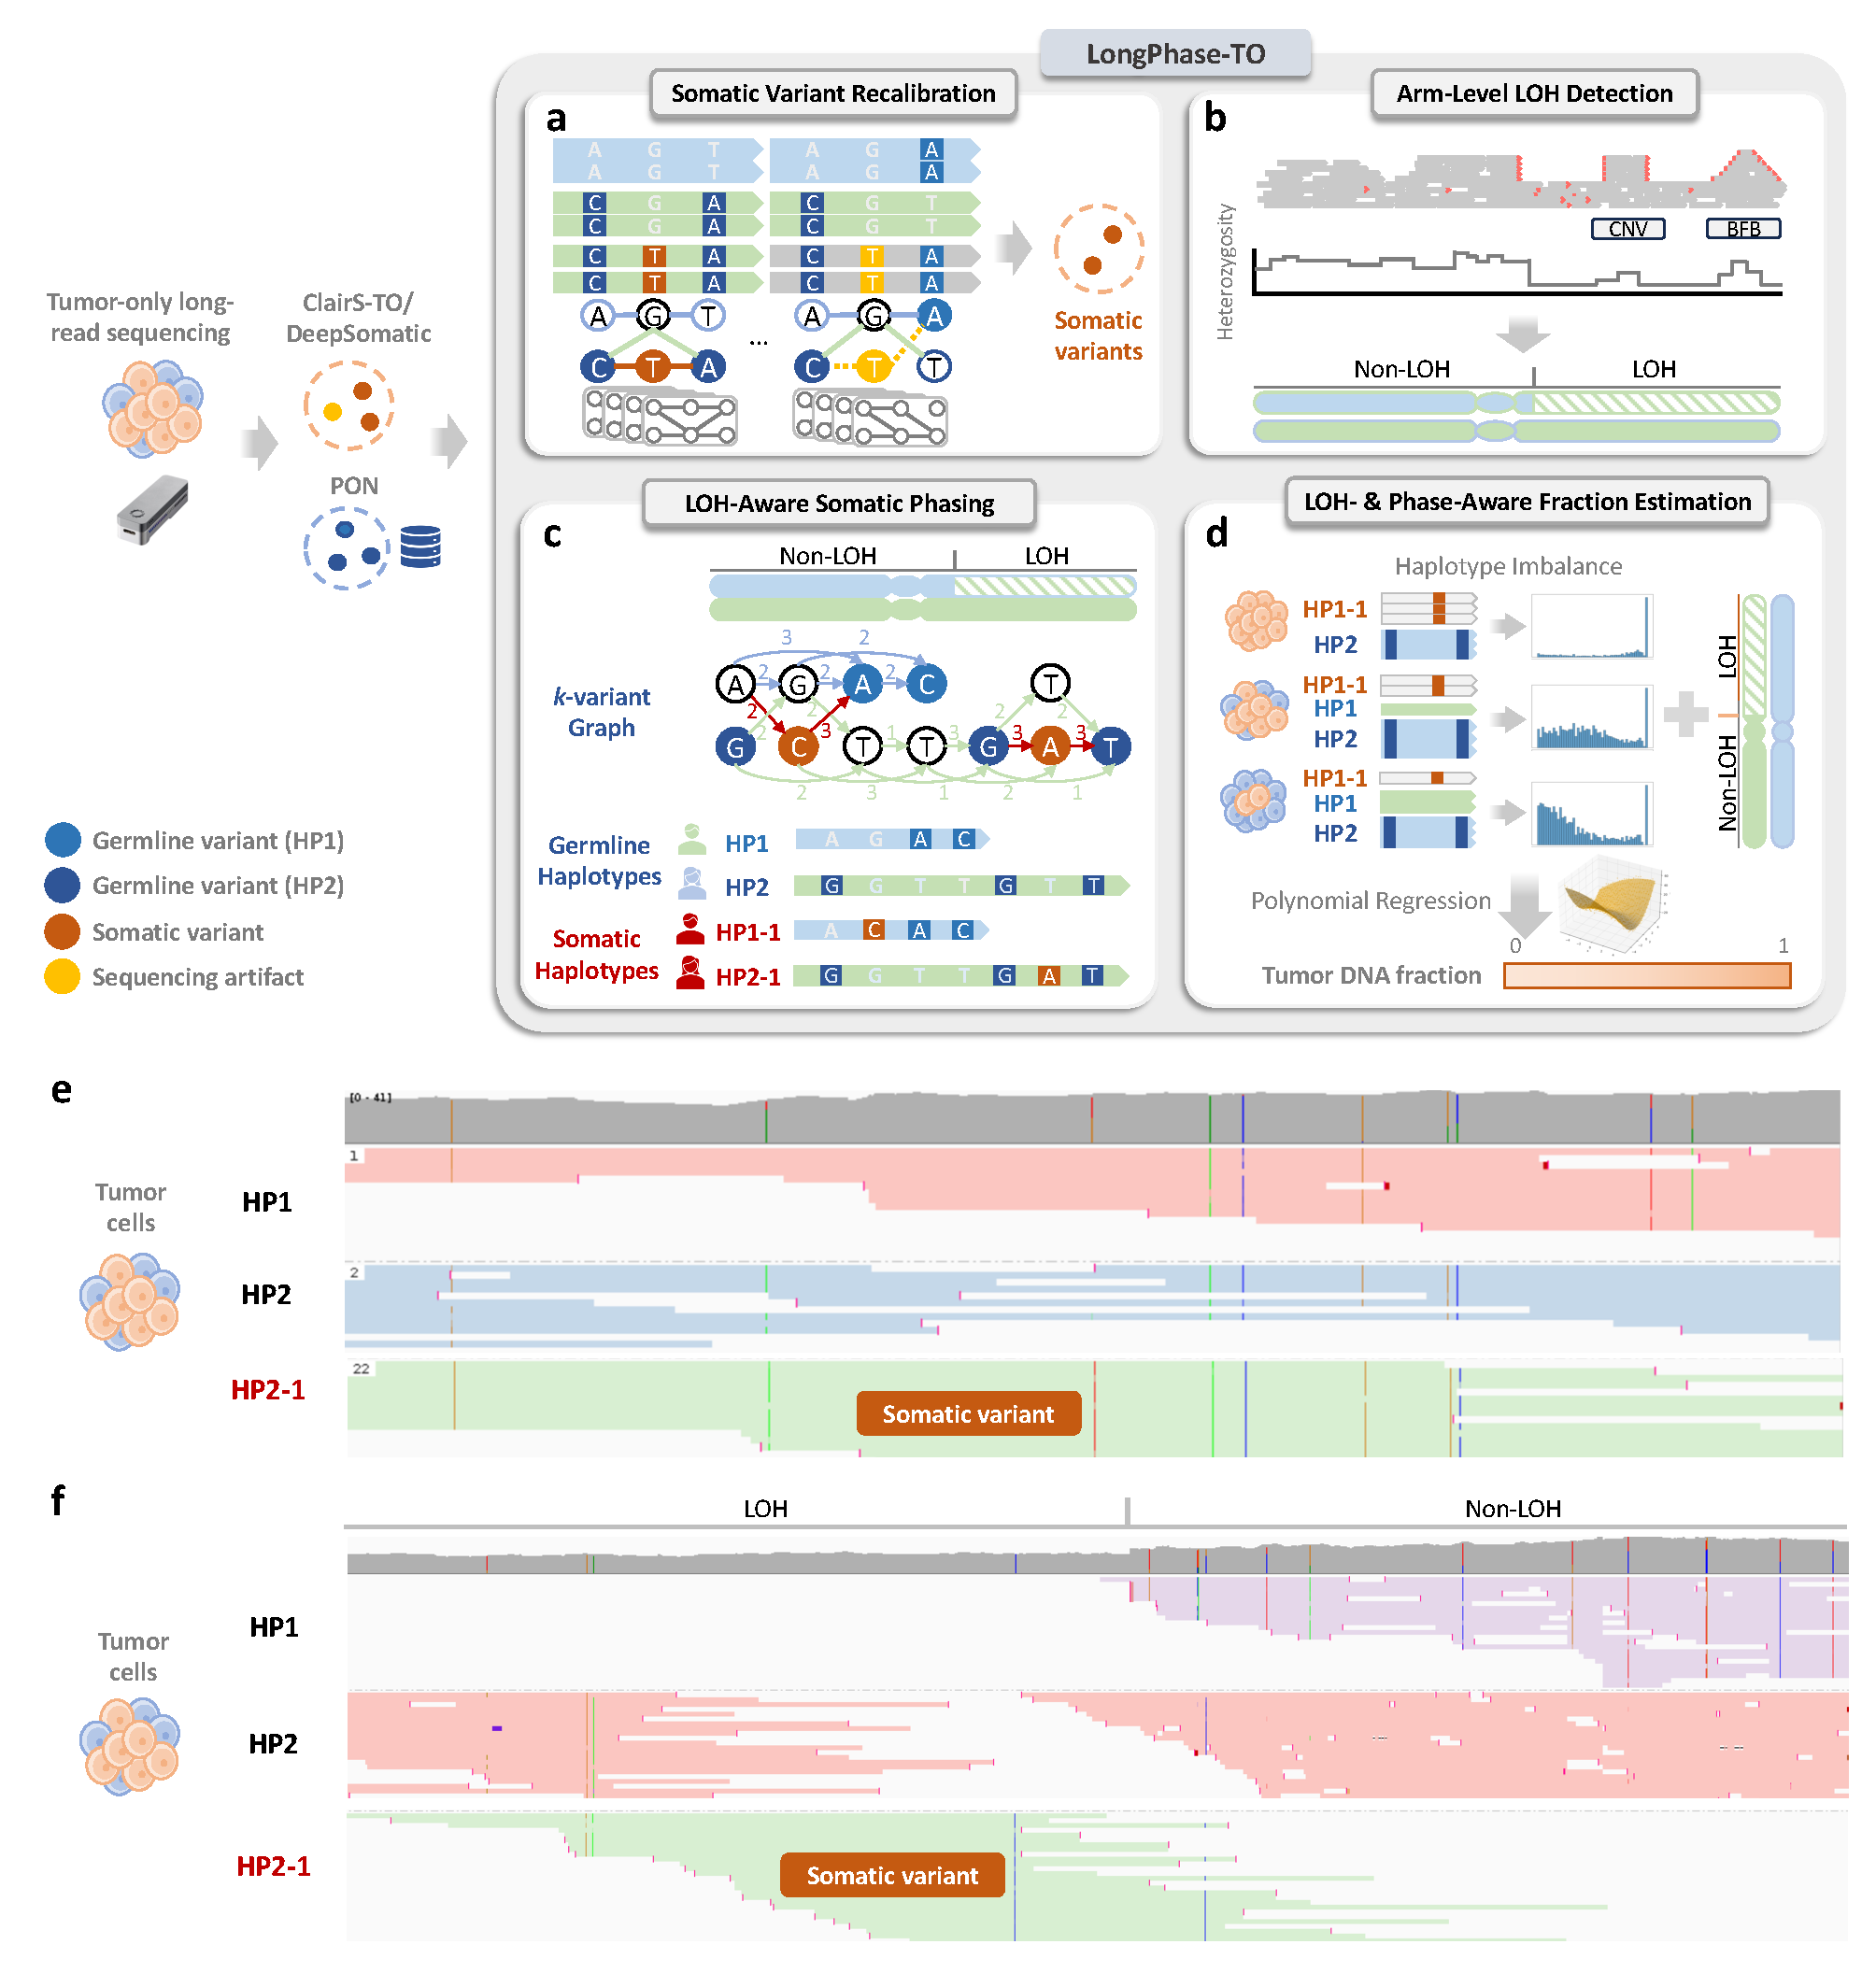
\includegraphics[width=\linewidth,height=0.78\textheight,keepaspectratio]{Figure_1.pdf}
    \caption{
      Overview of the LongPhase-TO somatic haplotype phasing framework.
      (a) Haplotype-aware recalibration refines initial somatic variant calls from ClairS-TO or DeepSomatic-TO by integrating PoNs and haplotype linkage information, distinguishing true somatic variants (orange) from sequencing artifacts (yellow) and germline variants (blue).
      (b) Chromosome-scale LOH detection identifies large-scale allelic imbalances by analyzing CNV/BFB intervals and heterozygosity ratios to distinguish LOH from non-LOH regions.
      (c) Somatic phasing assigns somatic variants to their originating germline haplotypes (HP1, HP2) and reconstructs derived somatic haplotypes (HP1-1, HP2-1), spanning LOH regions.
      (d) Phasing-informed copy-number fitting estimates tumor DNA fraction and ploidy from read depth and haplotype-resolved allelic balance, with LOH segments constraining the DNA fraction.
      (e) Haplotagged reads at a somatic SNV in HCC1395\_HKU: reads are partitioned into the germline haplotypes HP1 and HP2 and the somatic haplotype HP2-1, which carries the somatic allele and descends from HP2.
      (f) Haplotagging across an LOH boundary in the same dataset: within the LOH segment (left), where HP1 is lost, somatic reads remain tagged HP2-1 rather than collapsing into HP2, and both parental haplotypes are recovered in the adjacent non-LOH region (right).}
      \label{Figure_1.pdf}
\end{figure}

\begin{figure}[p]
    \centering
    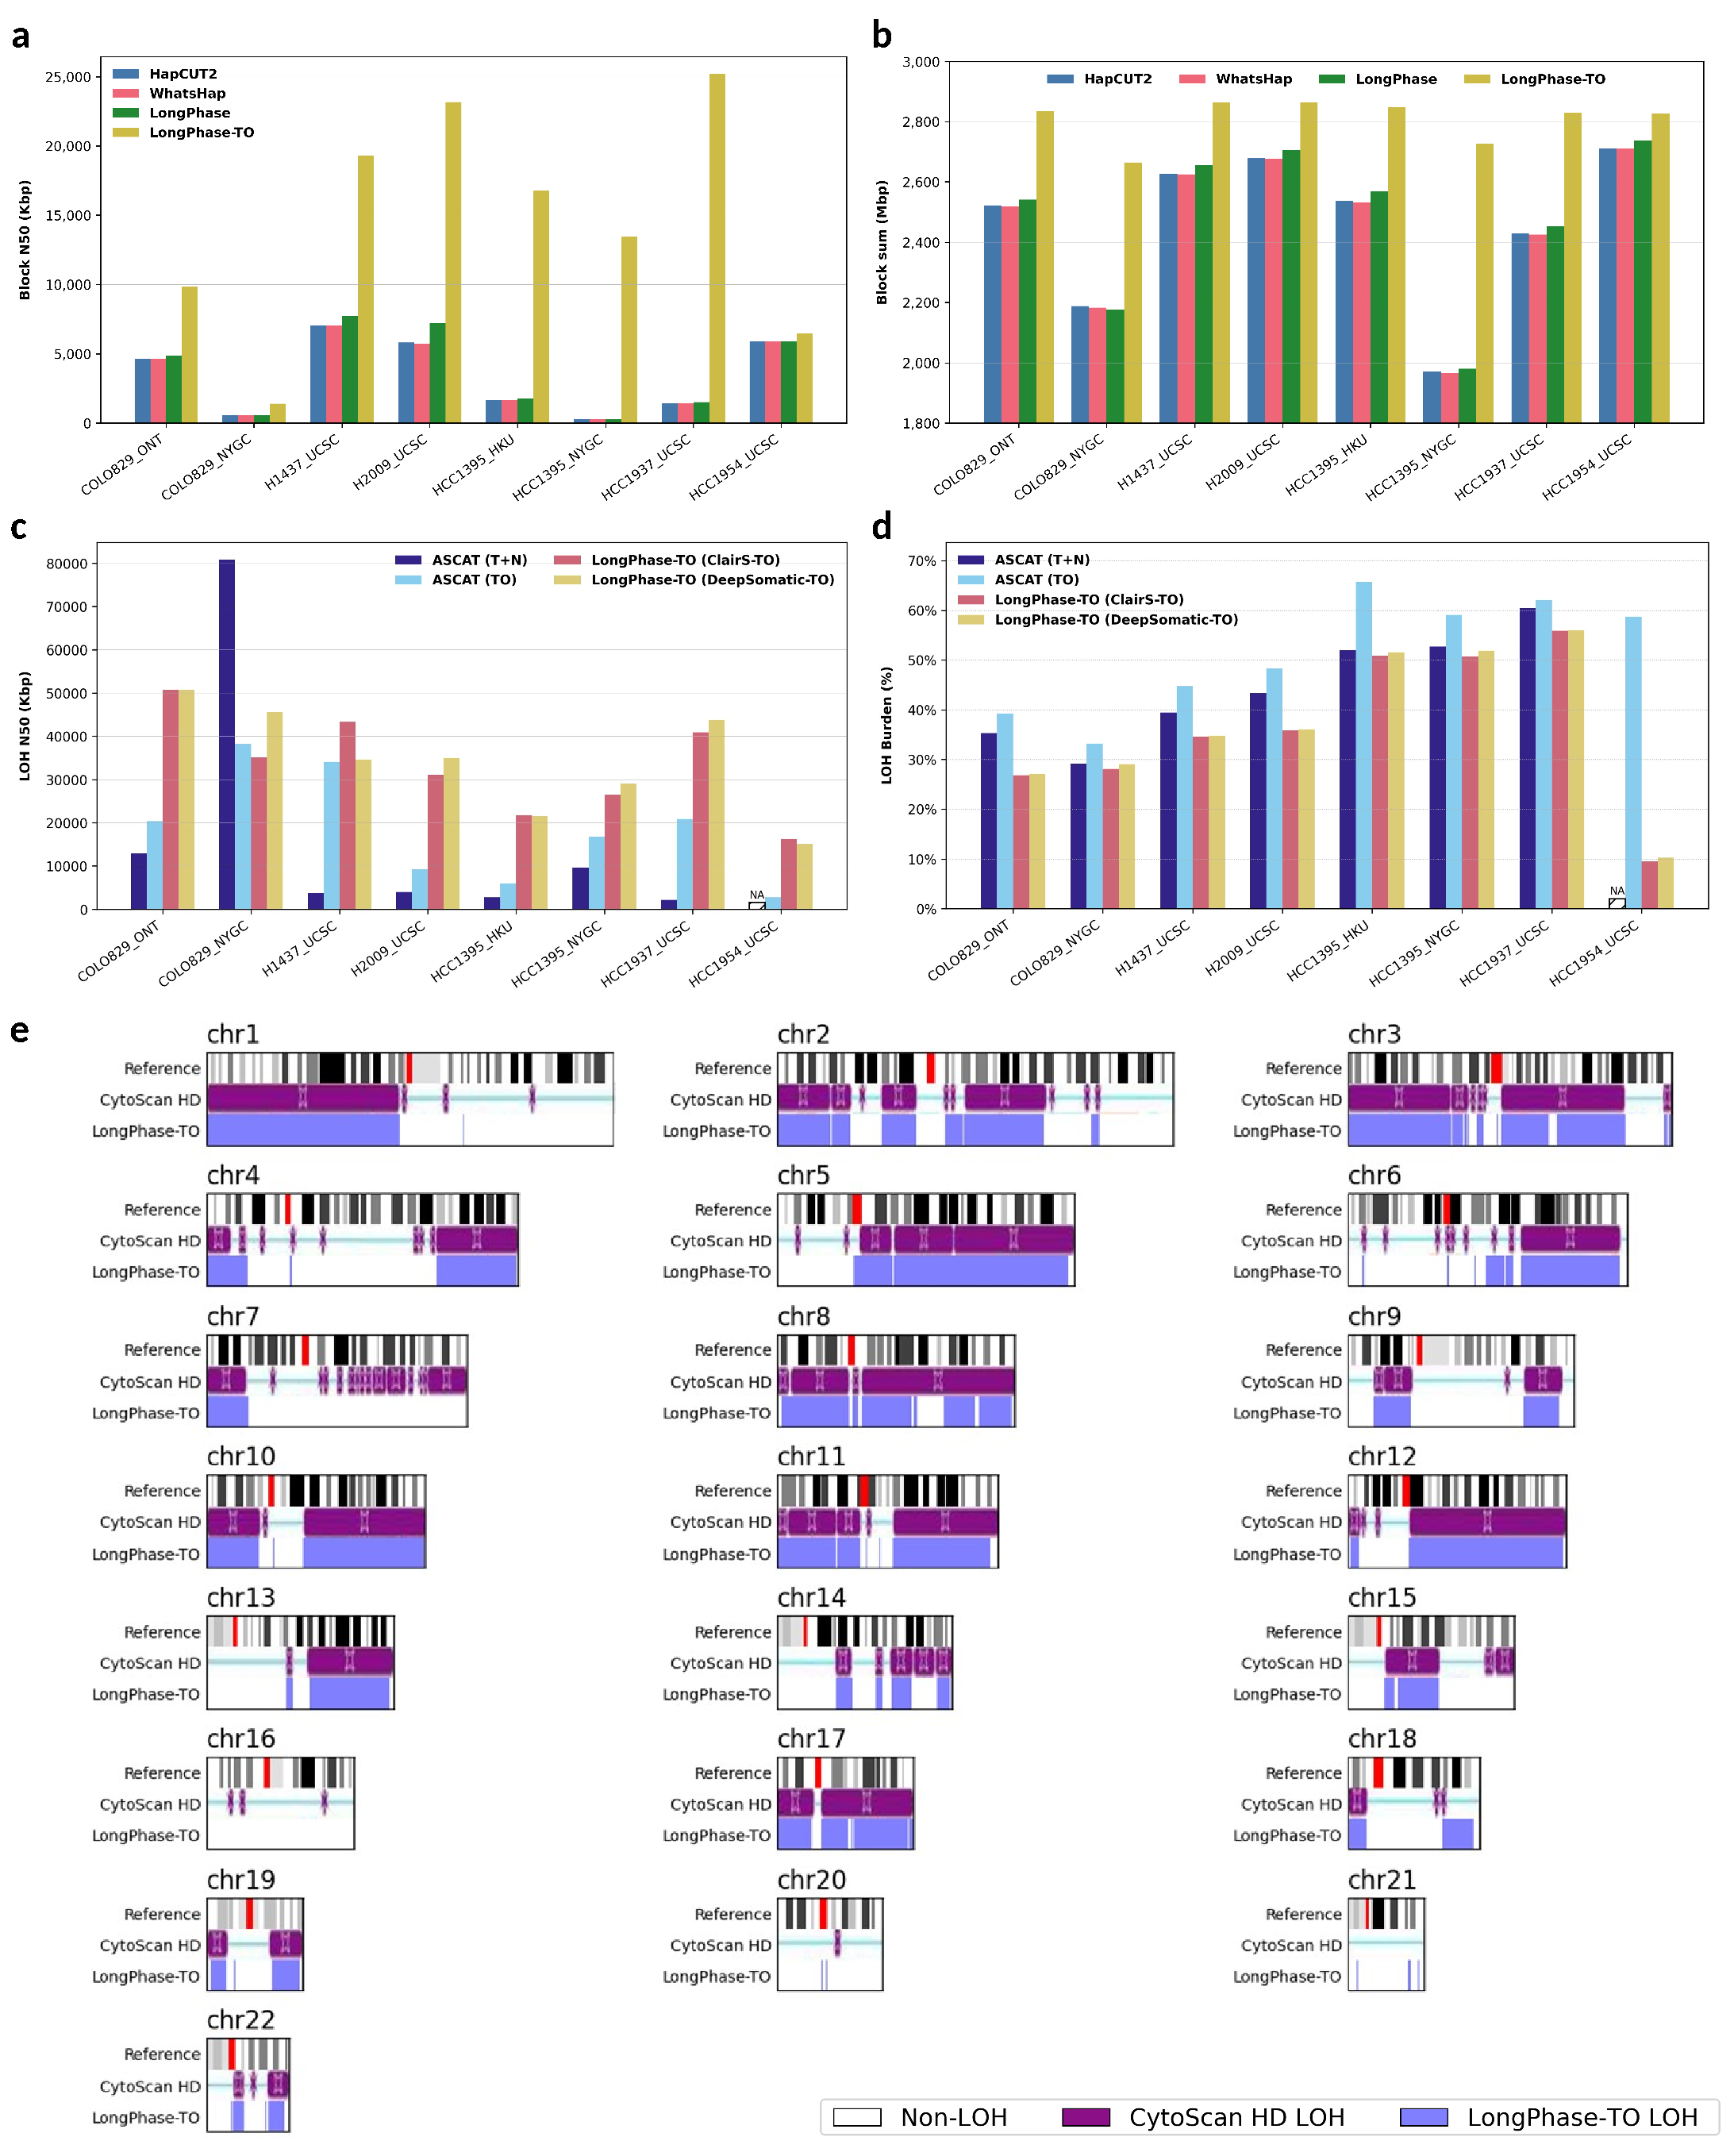
\includegraphics[width=\linewidth,height=0.78\textheight,keepaspectratio]{Figure_2.pdf}
    \caption{Comparison of LOH-aware phasing and LOH calling.
(a) Haplotype block N50 for three germline-based phasing tools (HapCUT2, WhatsHap, LongPhase) and the LOH- and somatic-aware phaser LongPhase-TO across eight datasets from six cancer cell lines.
(b) Total length of phased haplotypes for the same methods and datasets.
(c) LOH N50 of ASCAT in tumor-normal (T+N) and tumor-only (TO) modes and of LongPhase-TO using somatic variants from ClairS-TO or DeepSomatic-TO.
(d) LOH burden (fraction of the autosomal genome with LOH) of ASCAT (T+N), ASCAT (TO), and LongPhase-TO (ClairS-TO and DeepSomatic-TO).
(e) Orthogonal comparison in HCC1395, the only cell line with an available independent LOH profile: chromosome ideograms show reference cytobands (top), LOH segments reported by CytoScan HD microarray (middle, purple) and LOH segments inferred by LongPhase-TO (bottom, blue).}
    \label{Figure_2.pdf}
\end{figure}

\begin{figure}[p]
    \centering
    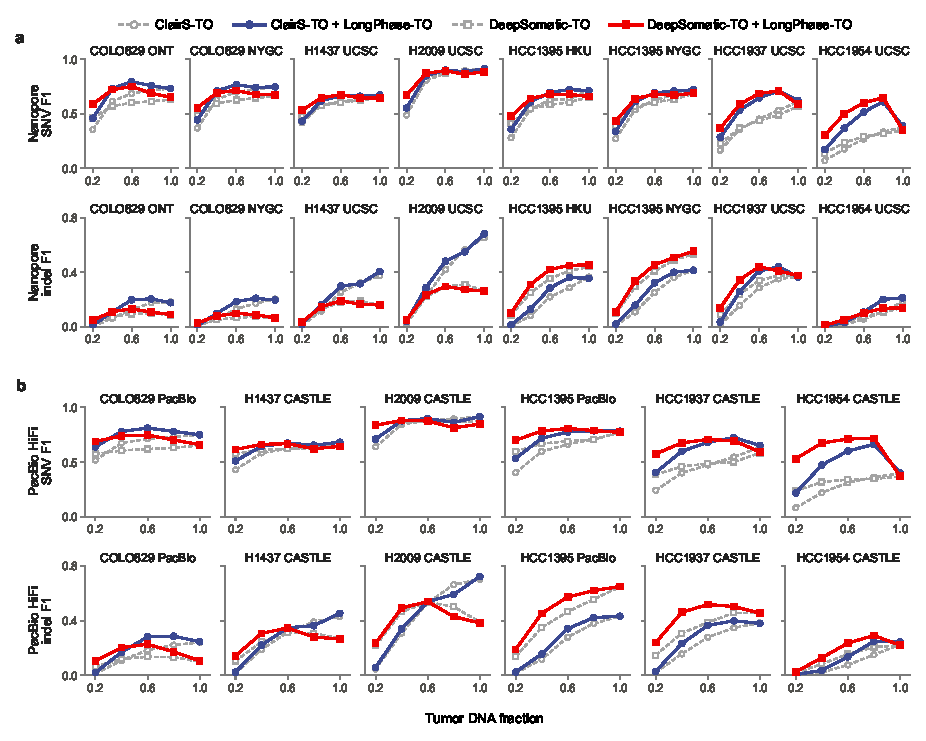
\includegraphics[width=\linewidth,height=0.78\textheight,keepaspectratio]{Figure_3.pdf}
    \caption{LongPhase-TO improves somatic SNV and indel calling on nanopore and PacBio HiFi data. (a) SNV (top) and indel (bottom) F1-score of ClairS-TO and DeepSomatic-TO at each tumor DNA fraction for the eight nanopore cell-line datasets. (b) The same for the six PacBio HiFi cell-line datasets. Solid colored lines show each caller with LongPhase-TO recalibration, and gray dashed lines show the caller alone (open circles for ClairS-TO and open squares for DeepSomatic-TO). The triplet-graph coefficients and thresholds were fitted on nanopore data and applied to PacBio HiFi data without refitting. DeepSomatic-TO with LongPhase-TO uses the ClairS-TO normal panels. Precision and recall of each dataset are shown in Supplementary Figures~\ref{fig:recal-ont-snv}, \ref{fig:recal-ont-indel}, \ref{fig:pacbio-snv-recalibration} and~\ref{fig:pacbio-indel-recalibration}.}
    \label{Figure_3.pdf}
\end{figure}

\begin{figure}[p]
  \centering
  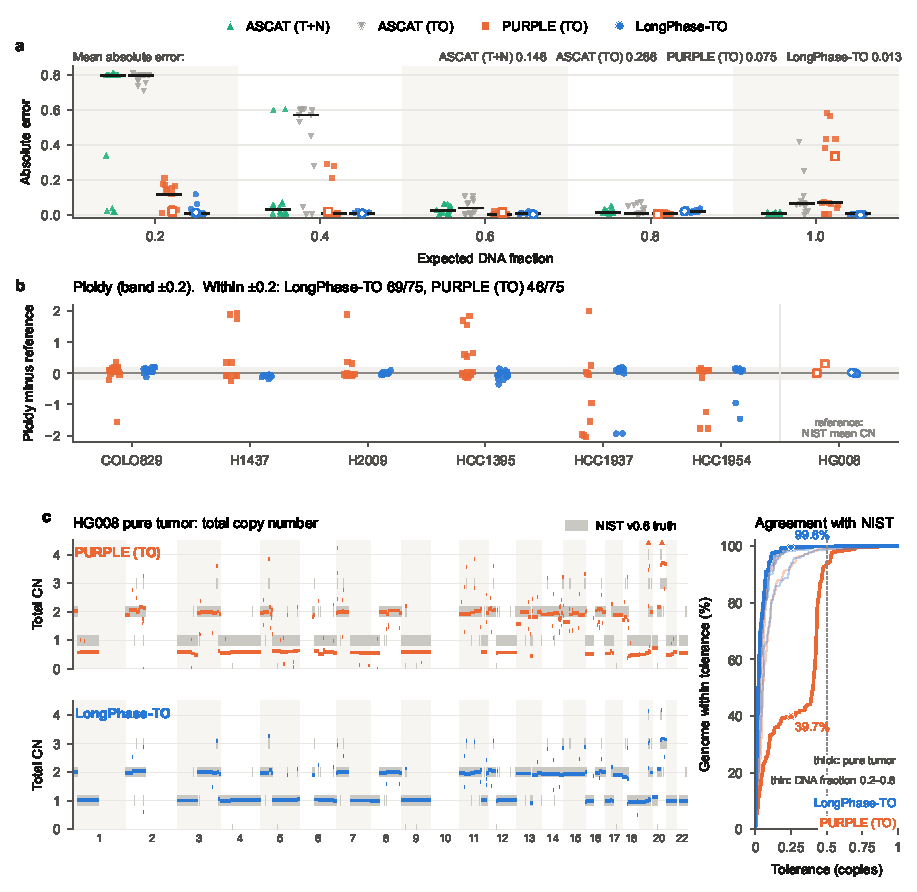
\includegraphics[width=\linewidth,height=0.78\textheight,keepaspectratio]{Figure_4.pdf}
  \caption{Phasing-informed estimation of tumor DNA fraction and ploidy.
(a) Absolute error of the estimated tumor DNA fraction at each expected fraction for ASCAT (T+N), ASCAT (TO), PURPLE (TO) and LongPhase-TO. Points are the eight nanopore and six PacBio HiFi cell-line dilution series and the five HG008 nanopore mixtures (open symbols). ASCAT was not run on HG008. Bars mark the median, and the numbers above the panel give the mean absolute error over all mixtures. ASCAT and PURPLE purities were converted to DNA fraction with each tool's fitted ploidy. Supplementary Figure~\ref{fig:pacbio-tdf} shows the estimates for each platform.
(b) Estimated ploidy minus reference ploidy for PURPLE (TO) and LongPhase-TO, for each cell line across all mixtures of both platforms. The reference is the published ploidy of each cell line and the NIST mean total copy number (1.47) for HG008. The band marks $\pm 0.2$.
(c) Total copy number of the pure HG008 tumor along chromosomes 1 to 22 for PURPLE (TO) (top) and LongPhase-TO (bottom), drawn over the NIST v0.6 benchmark (gray). Chromosome 10 has no truth. Triangles mark segments with a copy number above 4.5. Right, percentage of the evaluated genome whose estimated total copy number lies within a given tolerance of the NIST value, for the pure tumor (thick lines) and the four mixtures at expected DNA fractions of 0.2 to 0.8 (thin lines). Points mark a tolerance of 0.25 in the pure tumor.
LongPhase-TO values are from the DeepSomatic-TO configuration with the ClairS-TO normal panels.}
  \label{Figure_4.pdf}
\end{figure}

\end{document}
